\anonsection{Цель лабораторной работы}
Лабораторная работа №5 выполняется на основе лабораторной работы №4.
Целью лабораторной работы является освоение возможностей программы Microsoft Project по управлению финансовыми потоками на основе анализа затрат.

Команда разработчиков из 16 человек занимается созданием карты города на основе собственного модуля отображения. 
Проект должен быть завершен в течение 6 месяцев. Бюджет проекта: 50 000 рублей.

\anonsection{Индивидуальное задание}
Для выполнения лабораторной работы учитывались следующие параметры:
\begin{enumerate}
	\item Дата отчета: 25.04.2023.
	\item Задача <<Разработка 2D графических интерфейсов>> началась на 7 дней позже.
	\item Задача <<Разработка 3D графических интерфейсов>> закончилась на 7 дней позже.
	\item Задача <<Создание заставки>> выполнена на 90\%.
	\item С 1 апреля на неделю ведущего программиста отправили на курсы повышения квалификации, после чего его ЗП увеличилась на 5\%.
	\item Аренда сервера подорожала на 10\%, начиная с 10.04.2023.
	\item Начали проводиться презентации вместо совещаний раз в две недели (1 час), для которых нужны 4 листа А4 общей стоимостью в 50 рублей, в которых принимают участие только те сотрудники, у которых есть задачи на текущей неделе.
\end{enumerate}

\newpage
\anonsection{Задание 1}
Для анализа затрат проекта будет использоваться методика освоенного объёма.
Чтобы вывести таблицу с затратами проекта, требуется выбрать пункт \textit{Диаграмма Ганта с отслеживанием}, нажать сверху справа от таблицы, выбрать \textit{Освоенный объём}

На рисунке 1 представлена таблица метрик для проекта:
\FloatBarrier
\begin{figure}[h]	
	\begin{center}
		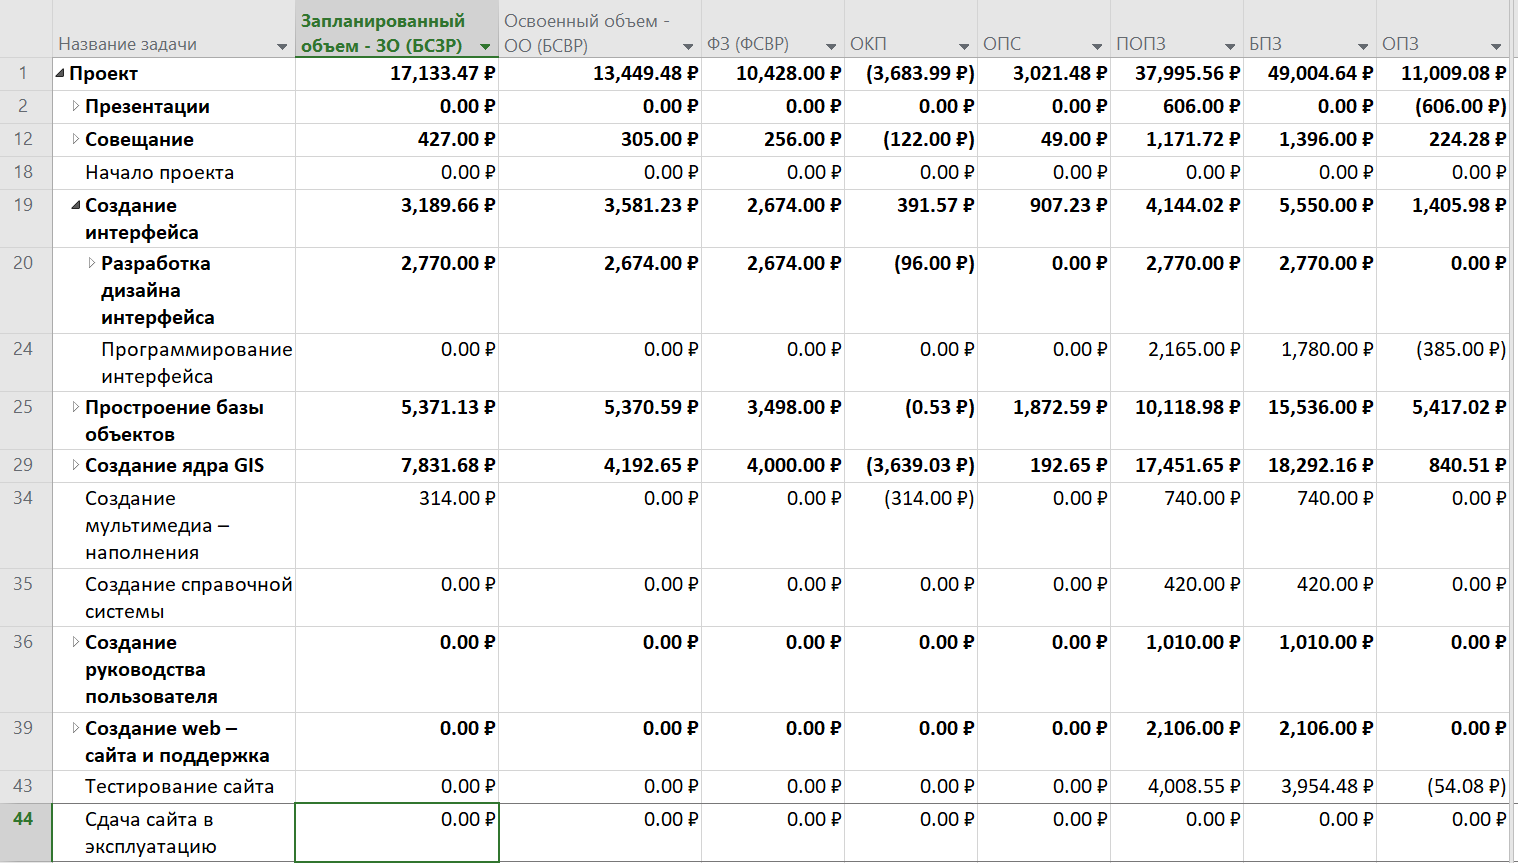
\includegraphics[width=\linewidth]{inc/task1.png}
	\end{center}
	\captionsetup{justification=centering}
	\caption{Освоенный объем проекта}
\end{figure}
\FloatBarrier 

В методику освоенного объёма входят следующие показатели:
\begin{itemize}
	\item \textbf{Запланированный объем} (ЗО) – средства, которые были затрачены на выполнение задачи в период с начала проекта до выбранной даты отчета, если бы задача точно соответствовала графику и смете.
	\item \textbf{Базовая стоимость выполненных работ} (БСВР) – средства, которые были затрачены на выполнение задачи с самого начала проекта до выбранной даты отчета, если бы фактически выполненная работа оплачивалась согласно смете, т.е. фактическое количество рабочих часов, оплачиваемых по сметным ставкам.
	\item \textbf{Фактические затраты} (ФЗ) – средства, которые были фактически потрачены на выполнение задачи в период с начала проекта до выбранной даты отчета, т.е. это фактическая стоимость или фактическая ставка, умноженная на фактические часы.
\end{itemize}

На основе этих показателей рассчитываются остальные параметры:
\begin{itemize}
	\item \textbf{Отклонение от календарного плана} (ОКП) – сравнительная характеристика сметной стоимости плановой и выполненной работы, которая позволяет вычислить несоответствие сметы, вызванное исключительно различиями между плановым и фактическим объемом работы.
	\item \textbf{Отклонение по стоимости} (ОКС) – сравнительная характеристика сметной и фактической стоимости выполненной работы, которая позволяет выделить несоответствие сметы, вызванное разницей стоимости ресурсов.
	\item \textbf{Предварительная оценка по завершению} (ПОПЗ) – в этом поле отображаются ожидаемые общие затраты для задачи, расчет которых основан на предположении, что оставшаяся часть работы будет выполнена в точном соответствии со сметой.
\end{itemize}

Анализируя проект методом освоенного объёма, можно сделать следующие выводы:
\begin{enumerate}
	\item Отклонение по стоимости проекта положительное -- это значит, затраты проекта находятся в пределах сметы.
	\item Отклонение по завершению положительное – средства не перерасходуются. Траты находятся в пределах нормы.
	\item Презентации позволили сократить затраты проекта, так как ОПЗ для презентаций составил -606 рублей, а для совещаний -- 1104 рубля.
	\item Из-за того, что для ведущего программиста была увеличена зарплата на 10\%, ОПЗ для тестирования сайта стало отрицательным, несмотря на то, что к задаче ещё никто не приступал.
\end{enumerate}

\anonsection{Задание 2}
Для того, чтобы провести анализ трат, требуется построить графики.
Это можно сделать в графе \textit{Отчёты}.

На графике представлено распределение трат в течение года:
\FloatBarrier
\begin{figure}[h]	
	\begin{center}
		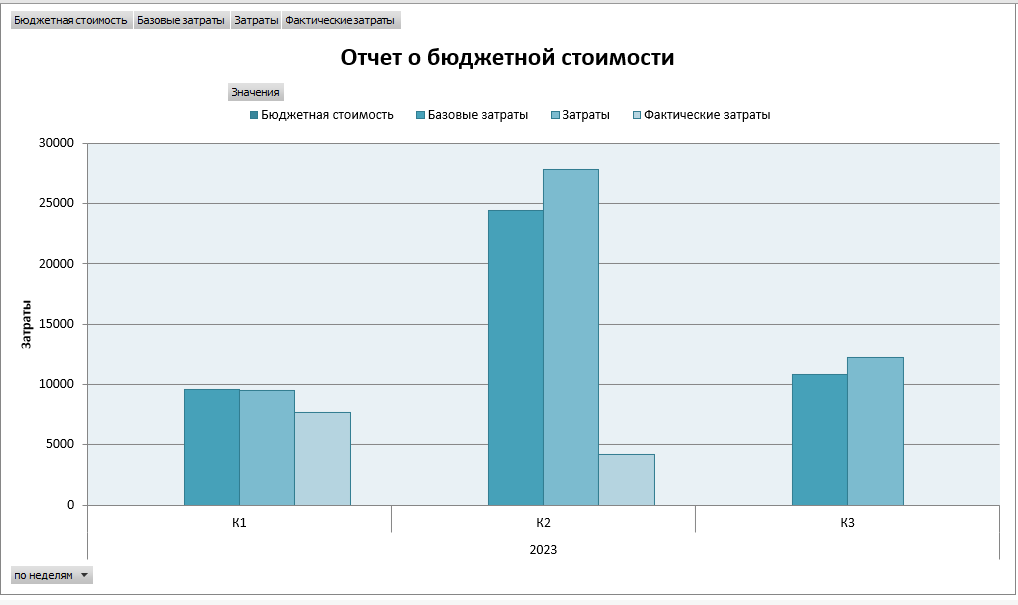
\includegraphics[width=\linewidth]{inc/budjet.png}
	\end{center}
	\captionsetup{justification=centering}
	\caption{Распределение трат в течение года}
\end{figure}
\FloatBarrier 

Как видно, львиная доля трудозатрат будет истрачена в середине проекта, так как в это время будут работать программисты.
При этом в первой трети будут работать более высокооплачиваемые специалисты, чем в конце, поэтому затрат больше, несмотря на то, что трудозатрат меньше в финальной трети.

\newpage
На графике представлен график превышения затрат для ресурсов:
\FloatBarrier
\begin{figure}[h]	
	\begin{center}
		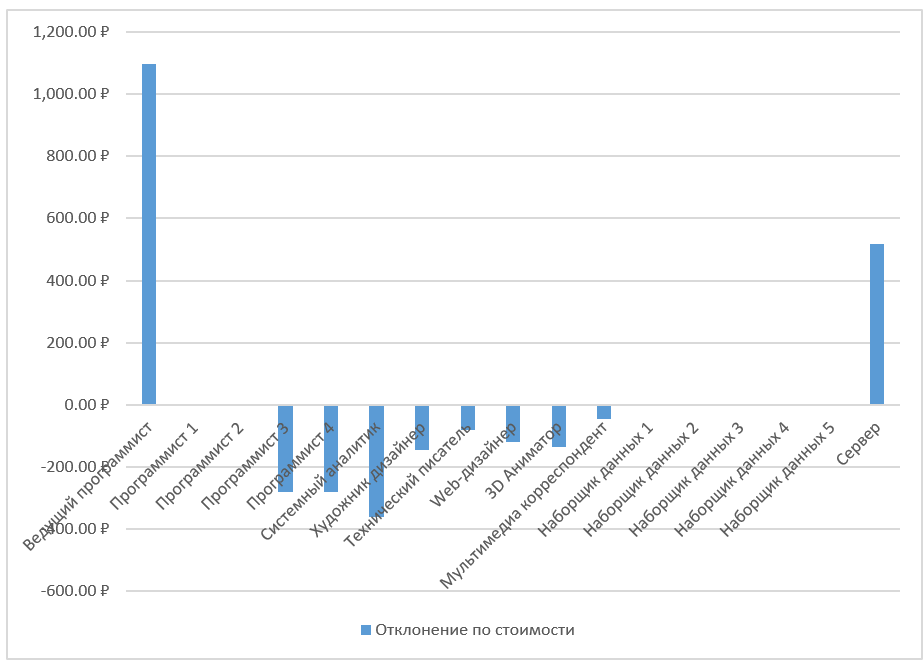
\includegraphics[width=\linewidth]{inc/graphResourses.png}
	\end{center}
	\captionsetup{justification=centering}
	\caption{График превышения затрат для ресурсов}
\end{figure}
\FloatBarrier 

Затраты на сервер и ведущего программиста оказались выше, что связано с индивидуальным заданием. 
Для всех остальных специалистов траты уменьшились из-за того, что были отменены совещания.
На программистов потрачено меньше, так как на одну из задач к ним был привлечен ведущий программист, что позволило уменьшить время реализации проекта.

\newpage
График превышение затрат для задач представлен на рисунке:
\FloatBarrier
\begin{figure}[h]	
	\begin{center}
		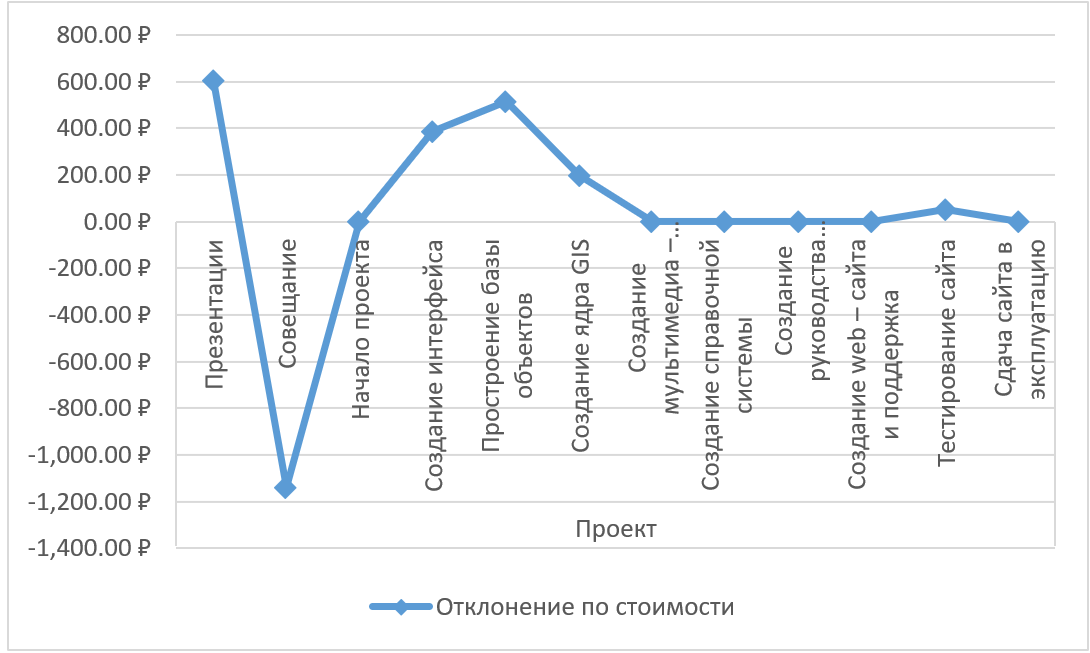
\includegraphics[width=\linewidth]{inc/listTasks.png}
	\end{center}
	\captionsetup{justification=centering}
	\caption{График превышения затрат для задач}
\end{figure}
\FloatBarrier 

Из них видно, что повысились траты за задачи, где используется сервер и ведущий программист: плата за них увеличилась.
Также увеличились траты на первые задачи, так как там произошла задержка.

\newpage
\anonsection{Задание 3}
В качестве декомпозиции для проекта были выполнены следующие меры:
\begin{itemize}
	\item Задачи <<Разработка руководства пользователя>> и две предыдущие были объединены в одну большую задачу -- <<Разработка UI для пользователей>>.
	Для реализации этих задач требуется лишь <<Разработка дизайна интерфейсов>>, соответственно, представители творческих профессий могут работать без перерыва.
	В дальнейшем, если потребуется, их можно будет не привлекать к совещанием, так как они быстрее выполнят свою работу.
	\item Создание Web-сайта не требует того, чтобы вся backend-часть была готова, соответственно, можно во время работы аналитиков их отправить реализовать сайт.
	\item Программирование интерфейсов не требует полной реализации <<Создание ядра GIS>>: эти задачи лучше выполнять параллельно.
\end{itemize}

Структура задач до изменений представлена на рисунке:
\FloatBarrier
\begin{figure}[h]	
	\begin{center}
		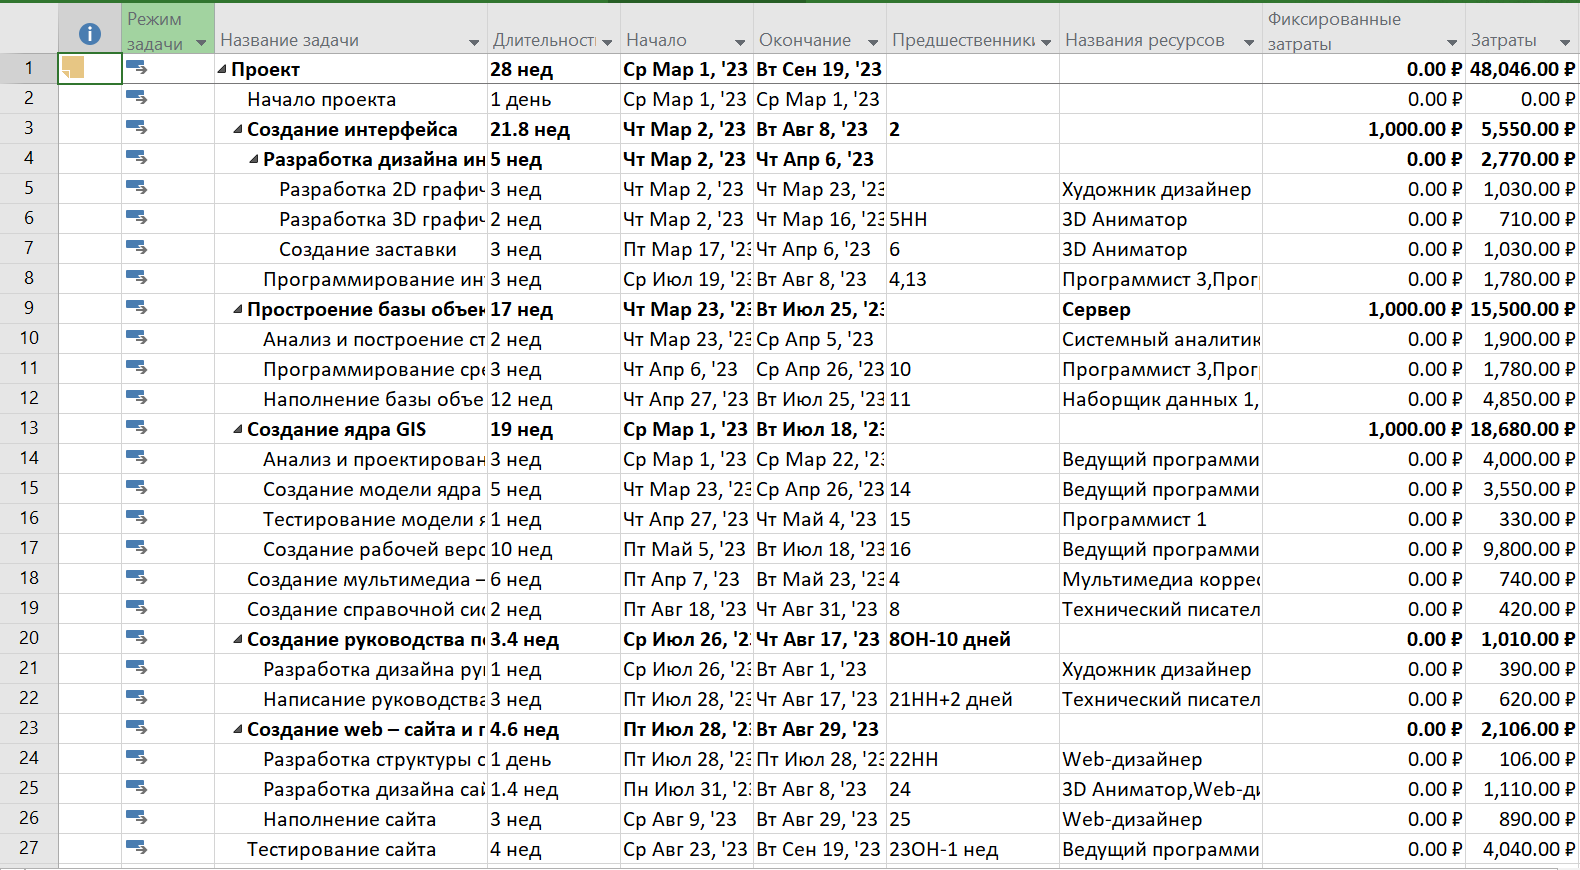
\includegraphics[width=\linewidth]{inc/before.png}
	\end{center}
	\captionsetup{justification=centering}
	\caption{Структура задач до изменений}
\end{figure}
\FloatBarrier 

Структура задач после изменений представлена на рисунке:
\FloatBarrier
\begin{figure}[h]	
	\begin{center}
		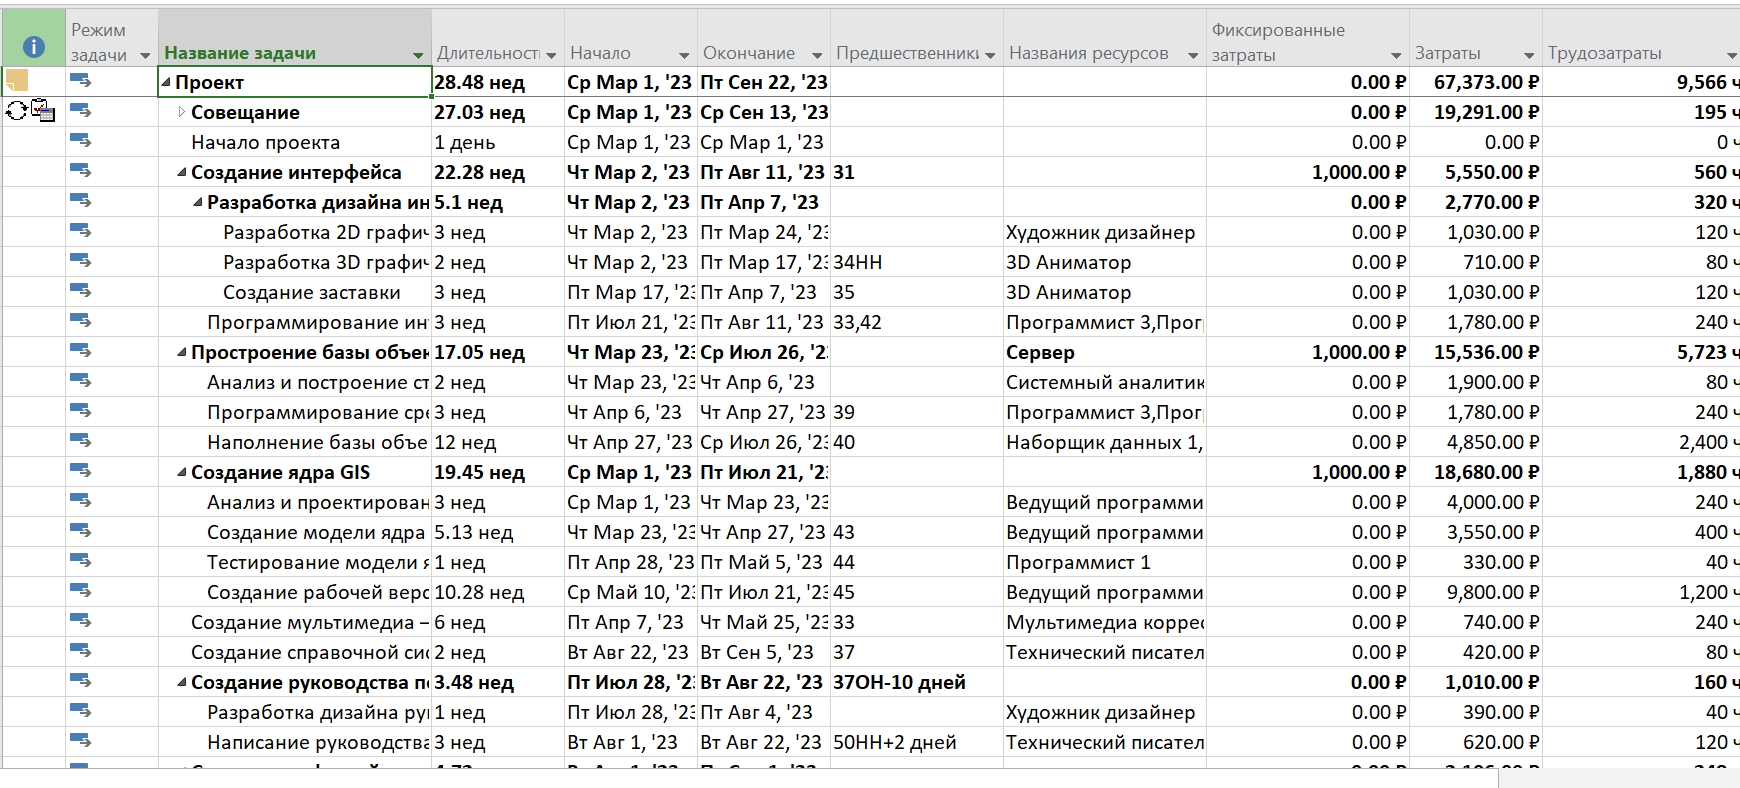
\includegraphics[width=\linewidth]{inc/after.png}
	\end{center}
	\captionsetup{justification=centering}
	\caption{Структура задач после изменений}
\end{figure}
\FloatBarrier 

Удалось сократить время реализации проекта на полтора месяца: с 19 сентября до 1 августа.
При этом бюджет составил 48546 рублей.

Круговая диаграмма затрат на ресурсы представлена на рисунке:
\FloatBarrier
\begin{figure}[h]	
	\begin{center}
		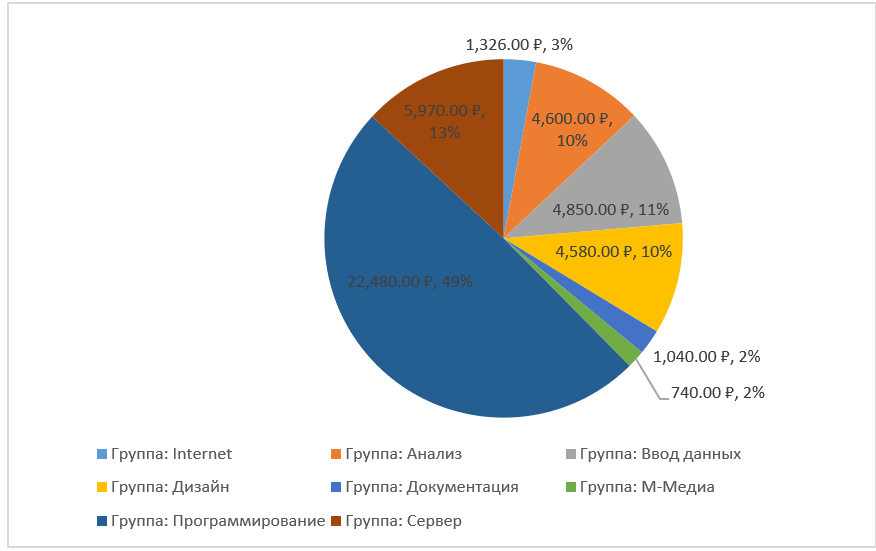
\includegraphics[height=7cm]{inc/result2.png}
	\end{center}
	\captionsetup{justification=centering}
	\caption{Затраты на группы ресурсов}
\end{figure}
\FloatBarrier 

\anonsection{Выводы}
В ходе выполнения данной лабораторной работы были освоены возможности программы Microsoft Project по управлению финансовыми потоками на основе анализа затрат.